\documentclass[12pt]{cover_letter}

\date{March 5, 2018}

\usepackage{pdfpages}

\begin{document}
  \begin{letter}{}

    \opening{Dear Tesla hiring manager,}

    % Sets the current page style to fancy (must happen after "opening")
    \thispagestyle{fancy}

    Your \textit{Prototype Engineering \& Fabrication Internship} posting found on the Tesla "Careers" website interests me. A background on extra-curricular competition teams has given me extensive experience in 3D CAD, design for manufacture, and rapid prototyping, which would allow me to make meaningful contributions on your product design team.

    I taught myself to use Dassault Solidworks as a seventh grader on a high school FIRST robotics team that had never used CAD before. Over the next six years, I improved my ability to rapidly ideate and design for ease of manufacture. Working with professional machine shops honed my ability to create unambiguous engineering drawings while the short, six-week build period taught me efficient design. In particular,  I became particularly adept in both designing for and manufacturing with our in-house manual mill, manual lathe, and Haas CNC router. By my senior year, each night I would design a prototype to solve a problem or test an idea, begin manufacturing on our CNC router at the next team meeting, and have a functioning concept by the meeting's conclusion. My skills would be invaluable to your team, where I could help create easy-to-manufature proofs of concept.

    My work at Georgia Tech has cemented my desire to use engineering principles to solve challenging problems. After I took Numerical Methods at GT, I wrote a Matlab script to create at optimal camshaft profile for my FSAE team's car. In the past year, I lead a team of six students in designing and manufacturing a three pound battlebot. The team extensively used FEA to optimize the chassis and weapon performance for their weight. I believe I would thrive on your collaborative, multi-disciplinary team where I would be challenged on a daily basis.

    Attached you will find my resume; it contains further descriptions of my work on Georgia Tech's FSAE and robotics teams and my high school robotics team. I would be happy to answer further questions by email at \href{mailto:michael.bick@gatech.edu}{\nolinkurl{michael.bick@gatech.edu}}.

    \closing{Sincerely,}

  \end{letter}

  % 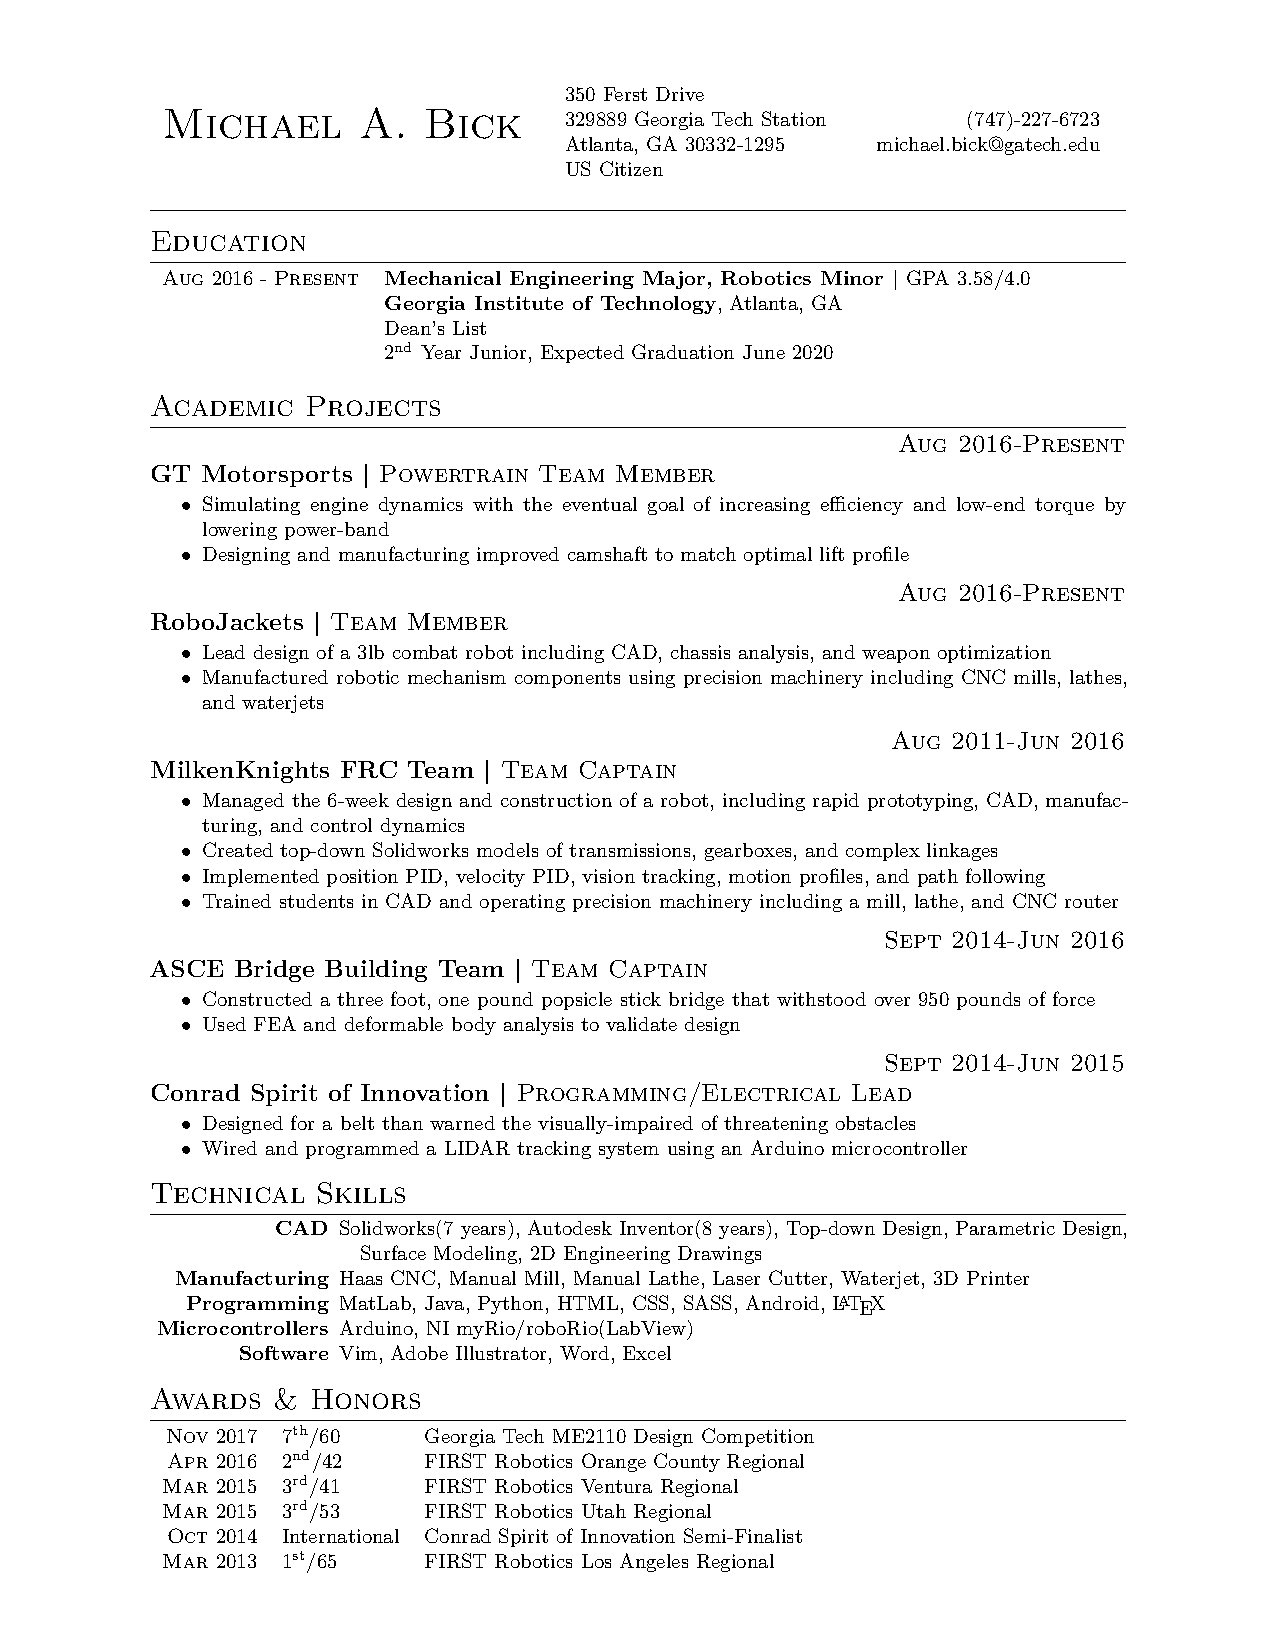
\includepdf[pages=-]{../../resumes/resume.pdf}
\end{document}
